\chapter{Proposed Method}
\label{chap:proposed-method}

This chapter presents \textbf{\gracefull{} (\gracename{})} by first defining
the heterogeneous multi-teacher distillation setting, then introducing the
\textbf{trie-Wasserstein KD loss}, \textbf{teacher routing network},
\textbf{gradient-agreement refinement mechanism} and \textbf{final training
objective}.

This chapter is organized as follows.
Section~\ref{sec:method-overview-formulation} introduces the problem
formulation and the overall \methodname{} training flow.
Section~\ref{sec:trie-wasserstein-distillation} presents trie-Wasserstein
distillation for mismatched tokenizers.
Section~\ref{sec:teacher-routing-network} defines the teacher routing network
and sparse top-\(k\) selection.
Section~\ref{sec:gradient-agreement-refinement} introduces gradient-agreement
refinement and the final teacher weighting mechanism.
Section~\ref{sec:final-objective} combines these components into the final
optimization objective.

\methodname{} addresses three core difficulties in heterogeneous
teacher-to-student VLM distillation. \textbf{First}, teacher and student models may use
different tokenizers and output vocabularies, so standard token-index KD is
not directly applicable. \textbf{Second}, teacher usefulness varies across
image-question pairs, making fixed teacher averaging inefficient. \textbf{Third}, even
routed teachers may still produce KD gradients that conflict with the
supervised task objective. \textbf{Finally}, the method developed in this chapter addresses
these issues through trie-Wasserstein KD, sparse teacher routing and
gradient-agreement refinement.

\section{Method Overview and Problem Formulation}
\label{sec:method-overview-formulation}

We consider multimodal understanding tasks that require reading image
text, understanding the question and generating an answer sequence
\cite{singh2019vqamodelsread,mathew2021docvqadatasetvqadocument,masry2022chartqabenchmarkquestionanswering}.
The training set is
\begin{equation}
\mathcal{D}=\{(x_n,y_n)\}_{n=1}^{N_{\mathrm{data}}},
\end{equation}
where \(x_n\) is a multimodal input and \(y_n\) is the target answer sequence.

Let \(S_{\theta}\) denote the student VLM with trainable parameters
\(\theta\), let \(G_{\phi}\) denote the trainable teacher router with
parameters \(\phi\) and let \(\mathcal{T}=\{T_i\}_{i=1}^{N}\) be the frozen
teacher pool. For each sample \(b\), the student produces logits
\(\mathbf{z}_s^{(b)}\) and teacher \(T_i\) provides teacher logits
\(\mathbf{z}_t^{(b,i)}\).
Throughout this chapter, the frozen teachers are treated as tokenizer-specific
experts: each teacher may use a different tokenizer, vocabulary and model
family and the router selects which experts contribute to each training
sample.

\methodname{} avoids a fixed teacher subset by learning
\textbf{sample-dependent sparse assignments} and refining the routed weights
with \textbf{parameter-gradient agreement}.

\begin{figure}[H]
\centering
\includegraphics[width=\linewidth]{figures/GRACE-Architecture.pdf}
\caption[GRACE architecture.]{GRACE architecture. The student produces logits and hidden states, the teacher routing network selects candidate teachers, trie-Wasserstein KD computes per-teacher losses and gradient-agreement refinement produces final KD weights.}
\label{fig:grace-architecture}
\end{figure}

Figure~\ref{fig:grace-architecture} summarizes the full training path. The
method is defined through four operators. \textbf{Trie-Wasserstein KD} computes
per-teacher distillation losses on a shared byte trie. The
\textbf{teacher routing network} selects candidate teachers from student-side
hidden states. \textbf{Gradient-agreement refinement} adjusts routed teacher
weights using parameter-gradient agreement. The \textbf{final objective}
combines supervised CE, routed KD and router auxiliary terms.

GRACE adapts sparse expert routing
\cite{shazeer2017outrageouslylargeneuralnetworks,fedus2022switchtransformersscalingtrillion}
to heterogeneous multi-teacher VLM distillation with token-level logit
supervision \cite{zhu2021studentcustomized}.

Table~\ref{tab:notation} summarizes the main notation used in the method.
Section~\ref{subsec:training-flow} gives a concise overview of one GRACE training update and the
following sections define these operators in detail, moving from
tokenizer-agnostic distribution matching to teacher routing,
gradient-agreement refinement and final loss aggregation.

\subsection{Notation}

\begin{table}[H]
\centering
\caption{Main symbols used in Chapter~\ref{chap:proposed-method}.}
\label{tab:notation}
\small
\begin{tabular}{@{}p{0.26\textwidth}p{0.66\textwidth}@{}}
\toprule
Symbol & Meaning \\
\midrule
\(\mathcal{D}=\{(x_n,y_n)\}_{n=1}^{N_{\mathrm{data}}}\) & Multimodal samples and target answer sequences. \\
\(S_{\theta}\), \(\mathcal{T}=\{T_i\}_{i=1}^{N}\) & Trainable student VLM and frozen teacher pool. \\
\(G_{\phi}\) & Trainable teacher routing network with parameters \(\phi\). \\
\(\mathbf{z}_s^{(b)}\), \(\mathbf{z}_t^{(b,i)}\) & Student and teacher logits for sample \(b\). \\
\(\mathbf{H}_s\), \(\mathbf{h}\) & Student hidden states and pooled routing feature. \\
\(T_{\mathrm{train}}\) & Total number of training steps. \\
\(\rho_{\mathrm{trie}}\), \(K_{\mathrm{TW}}\), \(e_{\mathrm{tail}}\) & Trie edge decay, sparse support size and residual tail edge. \\
\(k_{\mathrm{route}}\) & Configured router top-\(k\). \\
\(\mathbf{r}\), \(\mathbf{p}\) & Router logits and soft router weights. \\
\(\mathcal{C}_b\), \(\mathcal{R}_b\), \(\hat{\mathbf{p}}^{(b)}\) & Top-\(k\) candidate teacher set, routed teacher set and renormalized routed weights. \\
\(s_i\), \(\hat{s}_i\), \(\tilde{a}_i\), \(a_i^{(b)}\), \(\mathcal{A}_b\) & Raw agreement score, EMA-smoothed agreement score, teacher active flag, sample active flag and active routed set. \\
\(\boldsymbol{\omega}^{(b)}\), \(\mathbf{w}^{(b)}\) & Score-softmax weights and final KD weights. \\
\(\Omega_b^{CE}\), \(\Omega_{b,i}^{KD}\) & Supervised CE positions and matched KD positions. \\
\(\mathbf{g}_{CE}\), \(\mathbf{g}_i\) & CE and teacher-KD parameter gradients used by GRACE. \\
\(\beta_{\mathrm{EMA}}\), \(\beta_{\mathrm{score}}\), \(\epsilon_{\mathrm{num}}\), \(\epsilon_{\mathrm{fb}}\), \(\lambda_{\mathrm{blend}}\) & EMA decay, score-softmax sharpness, cosine stabilizer, fallback threshold and router-score blend exponent. \\
\(\mathrm{TopKRoute}\) & Sparse top-\(k\) teacher routing with routed-weight renormalization. \\
\(U\) & Uniform fallback weights over the active routed set. \\
\(\mathrm{Blend}\) & Mixing routed weights with GRACE score weights. \\
\(\mathrm{EMA}\) & Exponential moving average for GRACE scores. \\
\bottomrule
\end{tabular}
\end{table}

Each GRACE update can be viewed as a four-stage training flow:
\textbf{student forward pass}, \textbf{teacher routing},
\textbf{trie-Wasserstein KD computation} and
\textbf{gradient-agreement refinement}. In the first stage, the student
processes the mini-batch to produce answer-token logits \(\mathbf{z}_s\),
hidden states \(\mathbf{H}_s\) and the supervised loss
\(\mathcal{L}_{CE}\). The router then computes gate logits~\(\mathbf r\),
soft routing weights~\(\mathbf p\) and selects teachers with top-\(k\)
masking. The third stage computes per-sample, per-teacher trie-Wasserstein
losses \(\mathcal{L}_{KD}^{(b,i)}\), which provide tokenizer-agnostic KD
signals for the selected teachers. The final stage computes
parameter-gradient agreement scores, smooths them over time, blends them with
the routed weights and applies fallback when needed.

\subsection{Training Flow}
\label{subsec:training-flow}

A GRACE update starts from a mini-batch
\(\mathcal{B}=\{(x_b,y_b)\}_{b=1}^{B}\) and a frozen teacher pool
\(\mathcal{T}=\{T_i\}_{i=1}^{N}\). The student \(S_\theta\) first processes the
multimodal inputs and returns answer-token logits \(\mathbf{z}_s\), hidden
states \(\mathbf{H}_s\) and the supervised loss \(\mathcal{L}_{CE}\). The
supervised answer positions \(\Omega_b^{CE}\) define both the cross-entropy
loss and the pooling region used by the teacher router.

The router pools the student hidden states over supervised answer positions and
maps the resulting feature \(\mathbf{h}^{(b)}\) to teacher scores. After softmax
normalization, top-\(k_{\mathrm{route}}\) masking keeps a small routed teacher
set \(\mathcal{R}_b\) for each sample. The selected teacher weights are
renormalized to obtain \(\hat{\mathbf{p}}^{(b)}\). This stage replaces fixed
teacher averaging with sample-dependent teacher selection.

For each routed teacher, GRACE compares the student answer-token distribution
with the corresponding teacher distribution using trie-Wasserstein KD. In the
implementation used for the experiments, teacher logits are generated offline
and streamed during training, so the online update trains only the student and
router while the teachers remain frozen. This produces a per-sample,
per-teacher KD loss \(\mathcal{L}_{KD}^{(b,i)}\).

During warmup, the final KD weights are the renormalized router weights. After
warmup, GRACE computes a teacher-level agreement score by comparing the
supervised CE gradient with each teacher's batch-level KD gradient. The
agreement scores are smoothed with EMA, intersected with the routed teacher set
and converted into final sample-level KD weights. If no routed teacher passes
the agreement threshold, GRACE falls back to the router weights. If active
scores are nearly tied, it uses uniform active weights. Otherwise, it blends
router weights with gradient-agreement weights.

The mini-batch KD loss is the weighted average of the routed per-teacher losses.
The final objective combines supervised CE, routed trie-Wasserstein KD, router
entropy regularization and router z-loss. The next sections define these
components formally.

\section{Trie-Wasserstein Cross-Tokenizer Distillation}
\label{sec:trie-wasserstein-distillation}

\subsection{Supervised Answer Tokens}

We apply distillation only on \textbf{supervised answer tokens}, not on prompt
tokens.
For sample \(b\), let \(\Omega_b^{CE}\) denote the student positions whose labels
are not ignored. For each teacher \(T_i\), let \(\Omega_{b,i}^{KD}\) denote the
matched answer positions after masking ignored labels on both student and
teacher sides, removing EOS from the student or teacher answer span when configured
and truncating both spans to a common length.


This is a position-wise alignment approximation across tokenizers: after
answer-span preprocessing, the \(j\)-th student and teacher answer positions are
treated as corresponding positions. The trie-Wasserstein term handles
token-distribution mismatch at each matched position, but it does not perform a
separate byte-level sequence alignment.

\subsection{Shared Byte Trie}

For each sample \(b\), token position \(j \in \Omega_{b,i}^{KD}\) and teacher \(T_i\), let
\(\mathbf{z}_{s,j}^{(b)} \in \mathbb{R}^{V_s}\) be the student logits and
\(\mathbf{z}_{t,j}^{(b,i)} \in \mathbb{R}^{V_i}\) be the teacher logits.
The student and teacher probability distributions are
\begin{equation}
\mathbf{p}_{s,j}^{(b)}
=
\mathrm{softmax}\!\left(\frac{\mathbf{z}_{s,j}^{(b)}}{\tau_s}\right),
\qquad
\mathbf{p}_{t,j}^{(b,i)}
=
\mathrm{softmax}\!\left(\frac{\mathbf{z}_{t,j}^{(b,i)}}{\tau_t}\right),
\end{equation}
where \(\tau_s\) and \(\tau_t\) are the student and teacher temperatures.

Teacher and student vocabularies may differ, so direct token-index matching is
not feasible. GRACE instead maps decoded teacher and student token strings
into a \textbf{shared UTF-8 byte trie}. Tokens with common byte prefixes share
the same initial trie path, even when their tokenizer IDs differ.

Using UTF-8 bytes is a necessary design choice because it provides a fixed alphabet and exposes
tokenizer artifacts such as leading spaces, wordpiece prefixes and multimodal
special tokens. Character-level matching is less stable because the same
visible text can be stored with different Unicode code-point sequences.

For example, a string with a \textbf{leading space maps} to byte sequence
\([32,99,97,116]\), while \texttt{cat} maps to \([99,97,116]\). The trie
therefore treats the leading-space byte as an \textbf{explicit edge}, while
\textbf{preserving the subsequent byte sequence} for the underlying word.

Each token string is converted to a byte sequence and terminated with an EOS
sentinel. The EOS marker separates complete tokens from strict prefixes, so
tokens such as \texttt{doc} and \texttt{document} remain distinct leaves even
though they share an initial path.

Let \(e\) denote a normal byte-trie or EOS edge and let \(d(e)\) be its depth.
GRACE assigns edge weights
\begin{equation}
w(e)=\rho_{\mathrm{trie}}^{d(e)-1},
\label{eq:tw_edge_weight}
\end{equation}
where \(0<\rho_{\mathrm{trie}}<1\). The first edge from the root has weight
\(1\) and deeper edges decay geometrically. This makes shared prefixes cheaper
than unrelated byte paths while preserving a valid tree metric
\cite{takezawa2021supervisedtreewasserstein,peyre2019computationaloptimaltransport}.

Different tokenizers may stop at different depths, but they still share the
same byte-prefix edges when their decoded token strings overlap in byte-prefix
structure. The example in Figure~\ref{fig:grace-trie-shared} uses the pair
\texttt{document}/\texttt{receipt} and \texttt{doc}/\texttt{rece}.

\begin{figure}[H]
\centering
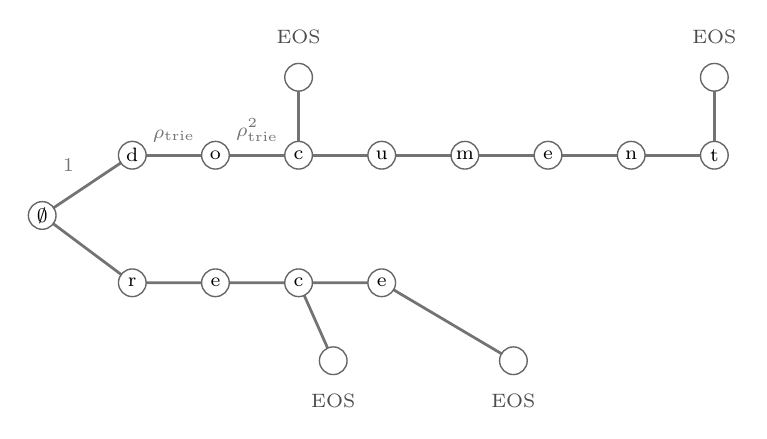
\begin{tikzpicture}[
    x=0.88cm,
    y=0.9cm,
    every node/.style={font=\small},
    every label/.style={fill=white, inner sep=1pt},
    triemark/.style={circle, draw=black!60, fill=white, line width=0.5pt, inner sep=0pt, minimum size=10pt},
    edge/.style={draw=black!55, line width=1.0pt}
]
    \coordinate (root) at (1.8, 2.4);
    \coordinate (d) at (3.1, 3.25);
    \coordinate (o) at (4.3, 3.25);
    \coordinate (c) at (5.5, 3.25);
    \coordinate (u) at (6.7, 3.25);
    \coordinate (m) at (7.9, 3.25);
    \coordinate (e) at (9.1, 3.25);
    \coordinate (n) at (10.3, 3.25);
    \coordinate (t) at (11.5, 3.25);

    \coordinate (r) at (3.1, 1.45);
    \coordinate (e2) at (4.3, 1.45);
    \coordinate (c2) at (5.5, 1.45);
    \coordinate (e3) at (6.7, 1.45);

    \coordinate (eosdoc) at (5.5, 4.35);
    \coordinate (eosdocument) at (11.5, 4.35);
    \coordinate (eosrece) at (6.0, 0.35);
    \coordinate (eosreceipt) at (8.6, 0.35);

    \draw[edge] (root) to node[midway, above left=1pt, font=\scriptsize, text=black!55] {1} (d);
    \draw[edge] (d) to node[midway, above=1pt, font=\scriptsize, text=black!55] {\(\rho_{\mathrm{trie}}\)} (o);
    \draw[edge] (o) to node[midway, above=1pt, font=\scriptsize, text=black!55] {\(\rho_{\mathrm{trie}}^2\)} (c);
    \draw[edge] (c) to (u) to (m) to (e) to (n) to (t);
    \draw[edge] (c) to (eosdoc);
    \draw[edge] (t) to (eosdocument);

    \draw[edge] (root) to (r) to (e2) to (c2) to (e3);
    \draw[edge] (c2) to (eosrece);
    \draw[edge] (e3) to (eosreceipt);

    \foreach \p/\lbl in {
        root/$\emptyset$, d/d, o/o, c/c, u/u, m/m, e/e, n/n, t/t,
        r/r, e2/e, c2/c, e3/e
    }{
        \node[triemark] at (\p) {\scriptsize \lbl};
    }

    \node[triemark, label={[font=\scriptsize, text=black!70, label distance=2mm]above:EOS}] at (eosdoc) {};
    \node[triemark, label={[font=\scriptsize, text=black!70, label distance=2mm]above:EOS}] at (eosdocument) {};
    \node[triemark, label={[font=\scriptsize, text=black!70, label distance=2mm]below:EOS}] at (eosrece) {};
    \node[triemark, label={[font=\scriptsize, text=black!70, label distance=2mm]below:EOS}] at (eosreceipt) {};

\end{tikzpicture}
\caption{Shared-trie view of tokenizer-mismatched matching for \texttt{document}/\texttt{receipt} and \texttt{doc}/\texttt{rece}.}
\label{fig:grace-trie-shared}
\end{figure}

Figure~\ref{fig:grace-trie-shared} illustrates this effect: shorter teacher
token sequences terminate earlier at EOS, whereas longer student token
sequences extend farther down the trie. As a result, the mismatch is
represented through the trie hierarchy instead of direct token-ID comparison.

\subsection{Trie-Wasserstein Objective}

The shared byte trie induces a tree metric over decoded token strings. Let
\(\mathcal{V}_s\) and \(\mathcal{V}_t\) denote the student and teacher token
vocabularies being compared at a given answer position and let \(\pi(v)\)
denote the trie path of decoded token \(v\). For an edge \(e\), the student
and teacher subtree masses are
\[
m_s(e)
=
\sum_{\substack{v\in\mathcal{V}_s\\ e\in\pi(v)}} p_s(v),
\qquad
m_t(e)
=
\sum_{\substack{u\in\mathcal{V}_t\\ e\in\pi(u)}} p_t(u).
\]
Thus, \(m_s(e)\) and \(m_t(e)\) measure how much probability mass each
distribution assigns to token paths passing through edge \(e\). The \(W_1\)
optimal transport distance between teacher and student token distributions on
the trie can then be written as a weighted sum of subtree-mass imbalances:
\begin{equation}
W_T(p_s,p_t)
=
\sum_{e\in E}
w(e)\left|m_s(e)-m_t(e)\right|.
\label{eq:trie-wasserstein-objective}
\end{equation}
This result follows from the standard \(W_1\) Kantorovich optimal transport
formulation under the trie-induced tree metric
\cite{peyre2019computationaloptimaltransport,takezawa2021supervisedtreewasserstein}.
The sparse construction below
applies the same formula to a bounded top-\(K_{\mathrm{TW}}\) support with a
residual tail edge.

\subsection{Sparse Support and Residual Tail Edge}

Equation~\eqref{eq:trie-wasserstein-objective} is exact on the complete shared trie, but
evaluating all vocabulary tokens at every answer position is expensive. GRACE
therefore applies the same subtree-mass formula on a \textbf{sparse augmented trie}.
For each aligned answer position, the method first masks ignored vocabulary
entries and retains the \textbf{top-\(K_{\mathrm{TW}}\) student and teacher tokens}.
These retained tokens are inserted into the shared UTF-8 byte trie while
preserving their exact trie paths and shared prefix structure. The probability
mass assigned to all remaining non-top-\(K_{\mathrm{TW}}\) tokens is not
discarded. Instead, it is collapsed into a single \textbf{residual tail edge}. The
trie-Wasserstein loss is then computed on the augmented structure containing
the retained token paths and the residual tail edge. This construction is
exact for the collapsed sparse trie, but it approximates the complete trie
distance because all omitted vocabulary mass is represented by one tail atom.

Let \(K_{\mathrm{TW}}\) denote the sparse trie support size. Let
\(\mathcal{V}_s^\star\) and \(\mathcal{V}_t^\star\) denote the non-ignored
student and teacher vocabularies. Before constructing the sparse trie, the
student and teacher probabilities are renormalized over the non-ignored
vocabularies so that the retained and residual masses form valid
distributions. Let
\(\mathcal{K}_{s,j}^{(b)}\subset\mathcal{V}_s^\star\) and
\(\mathcal{K}_{t,j}^{(b,i)}\subset\mathcal{V}_t^\star\) be the retained token
sets. The residual mass assigned to the tail edge is
\begin{equation}
r_{s,j}^{(b)}
=
1-\sum_{v\in\mathcal{K}_{s,j}^{(b)}}p_{s,j}^{(b)}(v),
\qquad
r_{t,j}^{(b,i)}
=
1-\sum_{v\in\mathcal{K}_{t,j}^{(b,i)}}p_{t,j}^{(b,i)}(v).
\end{equation}

Let \(\pi(v)\) be the trie path for token \(v\) and let
\(e_{\mathrm{tail}}\) be the global residual tail edge with
\(w(e_{\mathrm{tail}})=1\). For any active trie edge \(e\), the sparse subtree
masses are
\begin{equation}
m_{s,j}^{(b)}(e)
=
\sum_{\substack{v\in\mathcal{K}_{s,j}^{(b)}\\e\in\pi(v)}}
p_{s,j}^{(b)}(v)
\;+\;
\mathbf{1}[e=e_{\mathrm{tail}}]\,r_{s,j}^{(b)},
\end{equation}
\begin{equation}
m_{t,j}^{(b,i)}(e)
=
\sum_{\substack{v\in\mathcal{K}_{t,j}^{(b,i)}\\e\in\pi(v)}}
p_{t,j}^{(b,i)}(v)
\;+\;
\mathbf{1}[e=e_{\mathrm{tail}}]\,r_{t,j}^{(b,i)}.
\end{equation}
The token-level trie-Wasserstein loss is then
\begin{equation}
\ell_{TW}\!\left(\mathbf{z}_{s,j}^{(b)},\mathbf{z}_{t,j}^{(b,i)}\right)
=
\sum_{e\in\mathcal{E}_{act,j}^{(b,i)}}
w(e)\,
\left|
m_{s,j}^{(b)}(e)-m_{t,j}^{(b,i)}(e)
\right|,
\label{eq:token_tw}
\end{equation}
where \(\mathcal{E}_{act,j}^{(b,i)}\) contains the active student edges, active
teacher edges and the residual tail edge. Before the absolute value is applied,
\(m_{s,j}^{(b)}(e)-m_{t,j}^{(b,i)}(e)\) is positive when edge \(e\) carries more
student mass and negative when it carries more teacher mass.

The per-sample, per-teacher KD loss is the mean over supervised answer
tokens:
\begin{equation}
\mathcal{L}_{KD}^{(b,i)}
=
\frac{1}{|\Omega_{b,i}^{KD}|}
\sum_{j\in\Omega_{b,i}^{KD}}
\ell_{TW}\!\left(\mathbf{z}_{s,j}^{(b)},\mathbf{z}_{t,j}^{(b,i)}\right).
\label{eq:per_teacher_tw}
\end{equation}

The tail edge preserves probability mass outside the top-\(K_{\mathrm{TW}}\)
support without materializing every vocabulary path.

\paragraph{Complexity analysis.}
The shared byte trie is built once with time and memory cost
\(O(V_s \bar{L}_s + V_t \bar{L}_t)\), where \(V_s\) and \(V_t\) are the
student and teacher vocabulary sizes and \(\bar{L}_s\) and \(\bar{L}_t\) are
the average byte-path lengths. For one aligned answer position, extracting the
top-\(K_{\mathrm{TW}}\) student and teacher tokens costs
\(O(V_s\log K_{\mathrm{TW}} + V_t\log K_{\mathrm{TW}})\) with heap-based
selection. Given the retained token sets, sparse subtree-mass accumulation
walks only the retained token paths and the residual tail edge, costing
\(O(K_{\mathrm{TW}}\bar{L}_s + K_{\mathrm{TW}}\bar{L}_t + A)\), where \(A\)
is the number of active trie edges. If the implementation explicitly sorts or
deduplicates active edge indices, this adds an \(O(A\log A)\) term. Otherwise,
indexed accumulation gives an \(O(A)\) edge-aggregation cost.

Runtime memory is \(O(E + P_s + P_t + A)\), where \(E\) is the number of trie
edges and \(P_s\) and \(P_t\) are the stored student and teacher path-index
arrays. Unlike \textbf{dense OT}, the sparse computation does not materialize a
\(|V_s| \times |V_t|\) transport matrix.

Compared with the ULD baseline from Chapter~\ref{chap:preliminaries}, this
loss compares \textbf{mass on shared trie edges} instead of \textbf{ranked
logits}. It keeps the tokenizer-agnostic goal, but it uses a structured transport
view that is closer to the actual tokenizer geometry, while the
top-\(K_{\mathrm{TW}}\)+tail approximation keeps the cost bounded by the
retained support.

\begin{figure}[H]
\centering
\includegraphics[width=0.98\linewidth]{figures/grace_trie_sparse_tail.png}
\caption{Sparse trie-Wasserstein support and residual tail mass.}
\label{fig:grace-trie-sparse-tail}
\end{figure}

Figure~\ref{fig:grace-trie-sparse-tail} shows how the left and middle panels
keep top-\(K_{\mathrm{TW}}\) student and teacher tokens while assigning the
remaining probability to a residual tail edge. The right panel then compares
signed subtree masses on retained trie edges and the tail edge.

Table~\ref{tab:tw-vs-uld-toy} isolates the effect of \textbf{string geometry}.
Both rows have identical ranked masses, so \textbf{ULD gives the same value}.
Trie-Wasserstein assigns a lower loss to \texttt{doc}/\texttt{document} than
to \texttt{abc}/\texttt{def} because the former pair shares a
\textbf{byte prefix}.

\begin{table}[H]
\centering
\caption[Illustrative ULD and trie-Wasserstein comparison.]{Illustrative comparison between ULD and trie-Wasserstein under the same ranked masses. ULD assigns the same loss to both rows, while trie-Wasserstein gives lower loss to the pair with a shared byte prefix.}
\label{tab:tw-vs-uld-toy}
\small
\begin{tabular}{lcc}
\toprule
\textbf{Teacher / student top token} & \(\mathcal{L}_{ULD}\) & \(\ell_{TW}\) \\
\midrule
\texttt{doc} / \texttt{document} & 0.20 & 0.60 \\
\texttt{abc} / \texttt{def} & 0.20 & 3.29 \\
\bottomrule
\end{tabular}
\end{table}
\section{Teacher Routing Network}
\label{sec:teacher-routing-network}

\subsection{Router Architecture}

When multiple teachers are available, the method first builds a
\textbf{teacher routing network} instead of averaging them uniformly. The
router is applied to projector-based VLM students whose language-model head
exposes the text hidden width.

Let \(\mathbf{H}_s^{(b)}\) denote the student hidden states captured immediately
before the language-model head for sample \(b\). We pool these hidden states
over supervised answer positions to obtain a \textbf{routing feature}
\begin{equation}
\mathbf{h}^{(b)} = \mathrm{Pool}\!\left(\mathbf{H}_s^{(b)}\right).
\end{equation}
The pooling operation takes the mean over supervised answer positions. The
routing feature is defined for samples with at least one supervised answer
token, as ensured by the training data construction.

A learned MLP router \(G_{\phi}(\cdot)\) then produces gate logits
\begin{equation}
\mathbf{r}^{(b)} = G_{\phi}\!\left(\mathbf{h}^{(b)}\right).
\label{eq:router-logits}
\end{equation}
Soft routing weights are obtained by applying softmax to the router logits:
\begin{equation}
\mathbf{p}^{(b)} = \mathrm{softmax}\!\left(\mathbf{r}^{(b)}\right),
\label{eq:router-softmax}
\end{equation}
where \(p_i^{(b)}\) is the initial gate weight for teacher \(T_i\).
The gate stack uses LayerNorm, an up projection, a gate-value split, SiLU
gating and a down projection. The router then masks to the
top-\(k_{\mathrm{route}}\) teachers and renormalizes the selected softmax
weights.

\begin{figure}[H]
\centering
\includegraphics[width=\linewidth]{figures/deep-router.pdf}
\caption[Teacher routing network.]{Teacher routing network. Student hidden states are pooled over supervised answer positions, passed through a gated MLP router, converted into soft teacher weights and sparsified by top-\(k\) routing.}
\label{fig:deep-router}
\end{figure}

Figure~\ref{fig:deep-router} expands the teacher router used in the training
flow, showing the pooled student hidden state, gated MLP transformation,
softmax teacher weights and top-\(k\) sparsification step.



\subsection{Top-k Routing}

After computing soft routing weights, GRACE converts them into a
\textbf{sparse routed set}. For sample \(b\), GRACE first selects the highest-scoring teachers
according to the router logits:
\begin{equation}
\mathcal{C}_b=\mathrm{TopK}(\mathbf{r}^{(b)},\min(k_{\mathrm{route}},N)).
\end{equation}
The routed set is then defined as \(\mathcal{R}_b=\mathcal{C}_b\). All
non-selected teacher weights are set to zero and the remaining softmax
weights are renormalized. Let
\(m_i^{(b)}=\mathbf{1}[i\in\mathcal{R}_b]\) denote the top-\(k\) assignment
mask. The routed gate weights are
\begin{equation}
\hat{p}_i^{(b)}
=
\frac{m_i^{(b)} p_i^{(b)}}{\sum_{j=1}^{N} m_j^{(b)} p_j^{(b)}}.
\label{eq:constrained_gate_weights}
\end{equation}

The result is a \textbf{sparse routed teacher set} \(\mathcal{R}_b\) and
normalized \textbf{routed weights} \(\hat{\mathbf p}^{(b)}\), guaranteeing
that at least one teacher remains available before gradient-agreement
refinement.

\begin{figure}[H]
    \centering
    \includegraphics[width=0.78\linewidth]{figures/grace_routing_dynamics.png}
    \caption[Top-\(k\) routing dynamics in GRACE.]{Top-\(k\) routing dynamics in \methodname{}.}
    \label{fig:grace-routing-dynamics}
\end{figure}
Figure~\ref{fig:grace-routing-dynamics} contrasts the dense gate and routed
assignment view: the dense gate assigns nonzero probability to every teacher,
while top-\(k\) routing retains only the strongest candidates for each sample.
The logged assignment rate summarizes how often each teacher appears in the
routed set.

\subsection{Router Entropy and Z-Loss}

\methodname{} uses two auxiliary router terms to regularize the
teacher-selection mechanism. The first is \textbf{entropy regularization},
implemented as a negative-entropy term that discourages premature routing
collapse:
\begin{equation}
\mathcal{L}_{ent}
=
-\frac{1}{B}\sum_{b=1}^{B} H(\mathbf{p}^{(b)}).
\end{equation}
The second is the \textbf{router \(z\)-loss}, which keeps router logits
numerically well behaved:
\begin{equation}
\mathcal{L}_{z}
=
\frac{1}{B}\sum_{b=1}^{B}
\left(\log \sum_{i=1}^{N} e^{r_i^{(b)}}\right)^2.
\end{equation}
Neither term replaces the supervised CE or KD losses. They serve only to
stabilize routing behavior during training.
\section{Gradient-Agreement Refinement}
\label{sec:gradient-agreement-refinement}

As discussed in Section~\ref{subsec:gradient-conflict-teacher-agreement},
routed teachers may still conflict with the supervised objective after teacher
selection. \textbf{Gradient-agreement refinement} addresses this issue by
checking whether each selected teacher's KD direction agrees with the
supervised CE direction.

\subsection{Gradient Agreement Scoring}

Let \(\Theta\subseteq\theta\) denote the trainable student parameters used by the
optimizer. GRACE scores each teacher by comparing the
\textbf{supervised CE gradient} with each \textbf{teacher-specific KD
gradient} in student-parameter space. The CE gradient is
\begin{equation}
\mathbf{g}_{CE}
=
\nabla_{\Theta}\mathcal{L}_{CE}.
\end{equation}
For teacher \(T_i\), \methodname{} computes the KD gradient from that
teacher's mean KD loss over the full mini-batch:
\begin{equation}
\mathbf{g}_{i}
=
\nabla_{\Theta}
\left(
\frac{1}{B}\sum_{b=1}^{B}\mathcal{L}_{KD}^{(b,i)}
\right).
\end{equation}
In this thesis, \(\mathcal{L}_{KD}^{(b,i)}\) is the trie-Wasserstein loss from
Equation~\ref{eq:per_teacher_tw}. These gradients are used only to score teacher
compatibility. The final parameter update still uses the full loss in
Section~\ref{sec:final-objective}.
\subsection{Agreement Scores and Active Set}

For each teacher \(T_i\), GRACE measures directional agreement between
supervised learning and KD by cosine similarity:
\begin{equation}
s_i
=
\frac{
\langle \mathbf{g}_{CE},\mathbf{g}_i\rangle
}{
\max\!\left(\|\mathbf{g}_{CE}\|_2\|\mathbf{g}_i\|_2,\epsilon_{\mathrm{num}}\right)
}.
\end{equation}

The agreement score \(s_i\) is \textbf{teacher-level} within the current
mini-batch. The same teacher score is broadcast across samples. Sample
dependence enters later through the routed set \(\mathcal{R}_b\), routed
router weights \(\hat{\mathbf{p}}^{(b)}\) and active set \(\mathcal{A}_b\).

GRACE forms the active set by combining teacher-level agreement with
sample-specific routing. The teacher-level agreement score is first converted
into a binary teacher flag:
\begin{equation}
\tilde{a}_i = \mathbf{1}[s_i > \delta],
\end{equation}
where \(\delta\) is the GRACE threshold. This flag is then intersected with
the routed teacher set for each sample:
\begin{equation}
a_i^{(b)}=\mathbf{1}[i\in\mathcal{R}_b]\tilde{a}_i,
\qquad
\mathcal{A}_b=\{i\in\mathcal{R}_b:a_i^{(b)}=1\}.
\end{equation}

Thus, \(s_i\) is \textbf{teacher-level} within the mini-batch, while
\(\mathcal{A}_b\) remains \textbf{sample-specific} through
\(\mathcal{R}_b\). GRACE intentionally thresholds the current raw agreement
score. The score-softmax and fallback spread below use the EMA-smoothed score.

The agreement scores are used as non-differentiable routing statistics when
constructing the final KD weights. The final optimization step does not
backpropagate through the gradient-agreement computation itself.

\subsection{Warmup, EMA Smoothing and Score Weights}

The refinement stage uses \textbf{warmup}, \textbf{EMA smoothing} and
\textbf{score-softmax weighting} to stabilize teacher weights. Let
\(\rho_g \in [0,1]\) denote the GRACE warmup ratio relative to the total
number of training steps. During the first \(\rho_g T_{\mathrm{train}}\)
steps, GRACE leaves the routed gate weights unchanged:
\begin{equation}
w_i^{(b)}=\hat{p}_i^{(b)}.
\label{eq:grace_warmup_router_weights}
\end{equation}

After warmup, GRACE refines the routed teachers with a smoothed score
distribution. Let \(\bar{s}_i^{\mathrm{prev}}\) be the running exponential
moving average (EMA) of past batch means for teacher \(T_i\) and let
\(\beta_{\mathrm{EMA}}\) be the EMA decay. The smoothed score is
\begin{equation}
\hat{s}_i
=
\beta_{\mathrm{EMA}} \bar{s}_i^{\mathrm{prev}}
+
(1-\beta_{\mathrm{EMA}}) s_i.
\end{equation}

Smoothed scores produce more stable teacher weights, consistent with prior
findings on variance reduction in stochastic optimization.
If \(\mathcal{A}_b=\emptyset\), GRACE keeps the routed weights
\(\hat{\mathbf{p}}^{(b)}\). Otherwise, it converts smoothed scores into a
score-softmax weight vector over \(\mathcal{A}_b\):
\begin{equation}
\omega_i^{(b)}
=
\frac{
\exp(\beta_{\mathrm{score}}\hat{s}_i) \mathbf{1}[i \in \mathcal{A}_b]
}{
\sum_{j=1}^{N}
\exp(\beta_{\mathrm{score}}\hat{s}_j) \mathbf{1}[j \in \mathcal{A}_b]
},
\label{eq:grace_softmax}
\end{equation}
Here \(\beta_{\mathrm{score}}\) controls how sharply the highest-scoring active
teacher is preferred.

\subsection{Weight Blending and Fallback}

GRACE converts routed teacher scores into final KD weights through three
mutually exclusive cases.

\paragraph{No active teacher.}
If \(\mathcal{A}_b=\emptyset\), GRACE retains the routed weights:
\begin{equation}
w_i^{(b)}=\hat{p}_i^{(b)}.
\end{equation}

\paragraph{Low-confidence scores.}
If active teachers exist but their smoothed scores are too close, GRACE uses
uniform weights over the active set. The score range is
\begin{equation}
\Delta^{(b)}
=
\max_{i \in \mathcal{A}_b}\hat{s}_i
-
\min_{i \in \mathcal{A}_b}\hat{s}_i.
\end{equation}
If \(\mathcal{A}_b\neq\emptyset\) and
\(\Delta^{(b)} < \epsilon_{\mathrm{fb}}\), then
\begin{equation}
w_i^{(b)}
=
\frac{\mathbf{1}[i \in \mathcal{A}_b]}
{|\mathcal{A}_b|}.
\label{eq:alignment_fallback}
\end{equation}

\paragraph{Confident scores.}
Otherwise, GRACE blends router weights with score weights. Let
\(\lambda_{\mathrm{blend}} \in [0,1]\) be the router-blend exponent. The
unnormalized blended weights are
\begin{equation}
\tilde{w}_i^{(b)}
\propto
\left(\hat{p}_i^{(b)}\right)^{\lambda_{\mathrm{blend}}}
\left(\omega_i^{(b)}\right)^{1-\lambda_{\mathrm{blend}}},
\end{equation}
followed by normalization over the active routed teachers:
\begin{equation}
w_i^{(b)}
=
\frac{\tilde{w}_i^{(b)} \mathbf{1}[i \in \mathcal{A}_b]}
{\sum_{j=1}^{N}\tilde{w}_j^{(b)} \mathbf{1}[j \in \mathcal{A}_b]}.
\label{eq:effective_teacher_weights}
\end{equation}

Equations~\ref{eq:grace_softmax}, \ref{eq:alignment_fallback} and
\ref{eq:effective_teacher_weights} define the gradient-refinement operator.
The router first chooses \(\mathcal{R}_b\), GRACE filters it into the active
set \(\mathcal{A}_b\) and the final weights \(w_i^{(b)}\) are either
\textbf{inherited from the router}, \textbf{assigned uniformly under low score
spread}, or \textbf{obtained by a geometric blend} of \(\hat{p}_i^{(b)}\) and
\(\omega_i^{(b)}\). Figure~\ref{fig:grace-alignment-cases} shows these
weighting regimes.

\vspace{-0.4em}

\begin{figure}[H]
    \centering
    \includegraphics[width=\linewidth]{figures/grace_alignment_cases.png}
    \caption[Representative KD weighting regimes.]{Representative KD weighting regimes.}
    \label{fig:grace-alignment-cases}
\end{figure}

In all cases, \methodname{} only refines weights within the routed set, except
when no teacher passes the active threshold.

\subsection{Per-Sample KD Aggregation}

The \textbf{final KD loss for sample \(b\)} is the weighted sum of routed
per-teacher losses:
\begin{equation}
\bar{\mathcal{L}}_{KD}^{(b)}
=
\sum_{i\in\mathcal{R}_b} w_i^{(b)} \mathcal{L}_{KD}^{(b,i)}.
\label{eq:sample-kd-aggregation}
\end{equation}

The \textbf{mini-batch KD term} is
\begin{equation}
\mathcal{L}_{KD}
=
\frac{1}{B}\sum_{b=1}^{B}\bar{\mathcal{L}}_{KD}^{(b)}.
\label{eq:batch-kd}
\end{equation}

\section{Final Objective}
\label{sec:final-objective}

The preceding sections define the three components needed for the full
\methodname{} objective. First, \textbf{supervised CE} anchors the student to
ground-truth answer tokens. Second, \textbf{routed KD} transfers teacher
supervision after sparse routing and gradient-agreement refinement. Third,
\textbf{router regularization} stabilizes the teacher gate during training.

The final optimization objective is
\begin{equation}
\mathcal{L}
=
\mathcal{L}_{CE}
+
\alpha_{\mathrm{KD}}\mathcal{L}_{KD}
+
\lambda_{\mathrm{ent}}\mathcal{L}_{ent}
+
\lambda_{z}\mathcal{L}_{z},
\label{eq:final-objective}
\end{equation}

Here, \(\alpha_{\mathrm{KD}}\) controls the strength of teacher supervision
relative to the supervised answer-token loss. The coefficient
\(\lambda_{\mathrm{ent}}\) weights the entropy regularizer, which discourages
premature collapse of the teacher gate, while \(\lambda_z\) weights the router
\(z\)-loss, which keeps the gate logits numerically stable.

The objective is minimized with respect to \((\theta,\phi)\), where \(\theta\)
are the student parameters and \(\phi\) are the router parameters. All teacher
parameters remain frozen throughout training. In the experimental
implementation, teacher logits are generated offline and streamed during
training, so the online update does not require backpropagation through the
teacher pool.

During warmup, the KD weights are the renormalized top-\(k\) router weights.
After warmup, \methodname{} computes teacher-level gradient agreement, smooths
the scores with EMA and refines the KD weights within each routed teacher set.
Thus, routing acts as a candidate-selection mechanism, while gradient
agreement acts as a corrective weighting mechanism.

Equations~\eqref{eq:sample-kd-aggregation} through~\eqref{eq:final-objective}
specify how per-teacher losses are converted into the training loss used in
the experiments. The resulting objective addresses the three main difficulties
of heterogeneous multi-teacher distillation: trie-Wasserstein KD handles
tokenizer mismatch, sparse routing handles sample-dependent teacher utility
and gradient-agreement refinement suppresses routed teachers whose KD
gradients conflict with supervised learning.
